% EJC papers *must* begin with the following two lines. 
\documentclass[12pt]{article}
\usepackage{e-jc}

% Please remove all other commands that change parameters such as
% margins or pagesizes.

% only use standard LaTeX packages
% only include packages that you actually need

% we recommend these ams packages
\usepackage{amsthm,amsmath,amssymb}
\usepackage{verbatim}

% we recommend the graphicx package for importing figures
\usepackage{graphicx}

% use this command to create hyperlinks (optional and recommended)
\usepackage[colorlinks=true,citecolor=black,linkcolor=black,urlcolor=blue]{hyperref}

% use these commands for typesetting doi and arXiv references in the bibliography
\newcommand{\doi}[1]{\href{http://dx.doi.org/#1}{\texttt{doi:#1}}}
\newcommand{\arxiv}[1]{\href{http://arxiv.org/abs/#1}{\texttt{arXiv:#1}}}

% all overfull boxes must be fixed; 
% i.e. there must be no text protruding into the margins


% declare theorem-like environments
\theoremstyle{plain}
\newtheorem{theorem}{Theorem}
\newtheorem{lemma}[theorem]{Lemma}
\newtheorem{corollary}[theorem]{Corollary}
\newtheorem{proposition}[theorem]{Proposition}
\newtheorem{fact}[theorem]{Fact}
\newtheorem{observation}[theorem]{Observation}
\newtheorem{claim}[theorem]{Claim}

\theoremstyle{definition}
\newtheorem{definition}[theorem]{Definition}
\newtheorem{example}[theorem]{Example}
\newtheorem{conjecture}[theorem]{Conjecture}
\newtheorem{open}[theorem]{Open Problem}
\newtheorem{problem}[theorem]{Problem}
\newtheorem{question}[theorem]{Question}

\theoremstyle{remark}
\newtheorem{remark}[theorem]{Remark}
\newtheorem{note}[theorem]{Note}
\newcommand{\F}{\mathcal{F}}
\newcommand{\A}{\mathcal{A}}
\newcommand{\B}{\mathcal{B}}

%%%%%%%%%%%%%%%%%%%%%%%%%%%%%%%%%%%%%%%%%%%%%%%%%%%%%%%

% if needed include a line break (\\) at an appropriate place in the title

\title{\bf An Extension of a Result of Das-Gan-Sudakov}

% input author, affilliation, address and support information as follows;
% the address should include the country, and does not have to include
% the street address 

\author{Erik Waingarten\\
\small Department of Mathematics\\[-0.8ex]
\small Massachusetts Institute of Technology\\[-0.8ex] 
\small Cambridge, MA\\
\small\tt eaw@mit.edu\\
\and
Fermi Ma\\
\small Department of Mathematics\\[-0.8ex]
\small Massachusetts Institute of Technology\\[-0.8ex]
\small Cambridge, MA\\
\small\tt fermima@mit.edu
}

% \date{\dateline{submission date}{acceptance date}\\
% \small Mathematics Subject Classifications: comma separated list of
% MSC codes available from http://www.ams.org/mathscinet/freeTools.html}

\date{\dateline{August 1, 2014}{XX}\\
\small Mathematics Subject Classifications: XX}

\begin{document}

\maketitle

% E-JC papers must include an abstract. The abstract should consist of a
% succinct statement of background followed by a listing of the
% principal new results that are to be found in the paper. The abstract
% should be informative, clear, and as complete as possible. Phrases
% like "we investigate..." or "we study..." should be kept to a minimum
% in favor of "we prove that..."  or "we show that...".  Do not
% include equation numbers, unexpanded citations (such as "[23]"), or
% any other references to things in the paper that are not defined in
% the abstract. The abstract will be distributed without the rest of the
% paper so it must be entirely self-contained.

\begin{abstract}
  A result of Shagnik Das, Wenying Gan, and Benny Sudakov shows that

  % keywords are optional
  \bigskip\noindent \textbf{Keywords:} graph reconstruction
  conjecture; Broglington manifold; Pipletti's classification
\end{abstract}

\section{Introduction}

Let $B_n$ denote the poset of all subsets of $[n]$, where $F_1 \leq F_2$ if $F_1 \subseteq F_2$ as sets. A 2-chain is any pair of sets $F_1$ and $F_2$ such that $F_1 \subset F_2$. Sperner's Theorem states that any family of $B_n$ with no 2-chains has at most $\binom{n}{\lfloor n/2 \rfloor}$, a bound that can be shown to be tight by considering all the subsets of $[n]$ with size $\lfloor n/2 \rfloor$. Kleitman considered the related question of determining the minimum number of a 2-chains that must appear in a family of sets larger than $\binom{n}{\lfloor n/2 \rfloor}$. Das, Gan, and Sudakov considered this problem independently, and completely characterized all extremal families.

We analyze this problem for posets of the form $B_n / G$, where $G$ is subgroup of $S_n$.


%%%%%%%%%%%%%%%%%%%%%%%%%%%%%%%%%%%%%%%%%%%%%%%%%%%%%%%
\section{Notation}

%This section needs a lot of work

$B_n$ denotes the poset of all subsets of $[n]$, ordered by set inclusion. When we consider groups $G$, we say two elements $x, y$ of a set $S$ are in the same orbit if $\pi(x) = y$ for some $\pi \in G$. Thus, the orbits given by $G$ partition $S$ into disjoint, nonempty subsets. The set of all $G$-orbits of $S$ is denoted $S / G$, and in this paper we will consider the poset $B_n / G$ [Stanley]

%borrowed some wording from Stanley for the first paragraph. that needs to be fixed at some point.

We also use notation from [Das]. The $\ell$-shadow of a family is given by $\partial^{\ell}\F = \{G: \exists F \in \F, G \in F, |G| = |F| - \ell\}$.


%%%%%%%%%%%%%%%%%%%%%%%%%%%%%%%%%%%%%%%%%%%%%%%%%%%%%%%
\section{Groups Generated By a Transposition}

In this section, we restrict our attention to posets of the form $B_n / G$, where $G$ is a subgroup of the symmetric group $S_n$ on $n$ elements generated by a single transposition. WLOG, let the transposition be $(12)$, and denote by $G_{(12)}$ the two-element group generated by that transposition

Let the $i$th level of $B_n$ consist of all subsets $F$ of size $i$. Then Sperner's Theorem states that no antichain in $B_n$ is larger than the largest level $P_i$ [Stanley]. [Stanley] shows how to extend the theorem to $B_n / G$ for all groups $G$. 

The $i$th level of $B_n / G_{(12)}$ has size $\binom{n-2}{i-2} + \binom{n-1}{i}$, where the first term in the sum counts the number of sets that include both 1 and 2, while the second term counts the sets where at most one element of $\{1,2\}$ is included. Because $B_n / G$ is rank-symmetric, the largest level has $\binom{n-2}{\lfloor n/2 \rfloor -2} + \binom{n-1}{\lfloor n/2 \rfloor}$ elements, which is also the size of the largest family containing no 2-chains [Stanley]

%must add citations

Theorem 1.2 of [Das] completely characterizes the minimum number of 2-chains in families $\F$ of subsets of $B_n$. We present a similar result for families $\F$ of subsets of $B_n / G$, where $G$ is a group generated by a transposition. However, first we prove a lemma and a proposition.

\begin{lemma}
\[ \sum_{A\in \A}\sum_{i = 1}^{l-1} |U^i(M(A)) \cap \F| \leq \sum_{A \in \A}\sum_{i = 1}^{l-1} |\partial^i A | \]
when $l \leq 2m-1$
\end{lemma}

\begin{proof}
We first compute $L$ by spliting up $A$ in 2 cases:\\
1. $\{ 1, 2 \} \not\subset A$. In this case, whatever we chose to remove will get us a subset of $A$ that is below it. So the number of 2-chains lost involving this kind of $A$ is
\[ \sum_{i=1}^{l-1} \dbinom{\frac{n}{2} + m}{i} \]
2. $\{ 1, 2 \} \subset A$. In this case, it doesn't matter whether we remove $1$ or $2$, so we count the number of sets in the following manner. First, we assume that we remove either 1 or 2 or none. In the other case, we remove 1 and 2.
\[ \sum_{i=1}^{l-1} \left(\dbinom{\frac{n}{2} + m - 1}{i} + \dbinom{\frac{n}{2}+m-2}{i-2} \right) \]
So we have computed $L$ to be the sum over all $A \in \A$:
\[ L = \sum_{\{1, 2\} \not\subset A \in \A} \sum_{i=1}^{l-1} \dbinom{\frac{n}{2} + m}{i} + \sum_{\{1, 2\} \subset A \in \A} \sum_{i=1}^{l-1} \left( \dbinom{\frac{n}{2}+m-1}{i} + \dbinom{\frac{n}{2}+m-2}{i-2}\right) \]

Likewise, we can do the same for $G$, except now we are adding elements from the complements of $M(A)$. We can also assume that everything that we add is in $\F$ in the worst case
\[ G \leq \sum_{1 \in M(A) \text{ or } 2 \in M(A)} \sum_{i=1}^{l-1} \dbinom{\frac{n}{2}-m+l}{i} + \sum_{1, 2 \notin M(A)} \sum_{i=1}^{l-1} \left( \dbinom{\frac{n}{2}-m+l-1}{i} + \dbinom{\frac{n}{2}-m+l-2}{i-2} \right) \]

We know that $\dbinom{l}{k} > \dbinom{l-1}{k} + \dbinom{l-2}{k-2}$, so in order to show that 
\[ G \leq L \]
it sufficies to show that
\[ \dbinom{\frac{n}{2}-m+l}{i} \leq \dbinom{\frac{n}{2}+m-1}{i} + \dbinom{\frac{n}{2}+m-2}{i-2} \]
Which is true, since $l \leq 2m-1$.
\end{proof}

Now, let $m = \binom{n-2}{\lfloor n/2 \rfloor -2} + \binom{n-1}{\lfloor n/2 \rfloor}$.

\begin{proposition} For any $s > m$, there exists a family $\F$ of $s$ elements of $B_n / G_{(12)}$ that minimizes the number of 2-chains and is such that if $A \in \F$ is of maximal cardinality, where we write $|A| = \frac{n}{2}+m$, then for any $B \subset A$ with $|B| \geq \frac{n}{2} - m + 1$, $B \in \F$.
\end{proposition}

\begin{proof} Suppose this is false. We can assume $m \geq 1$ since if $m = 0$ there cannot be a subset $B$. Let $l \leq 2m-1$ be the minimal integer such that there exists a maximal cardinality set $A$ with a corresponding subset $l$ levels below that is not in $\F$. We define
\begin{align*}
\A &= \{A \in F| \lvert a \rvert = \frac{n}{2}+m, \partial^l A \not\subset \F \}\\
\B &= \partial^l A - \F
\end{align*}
Construct a bipartite graph on $\A \cup \B$ with an edge $(A,B)$ iff $B \subset A$. Each edge corresponds to a pair of sets that make the lemma false.

First, consider the case where there exists an injective mapping $M: \A \to \B$. We will show that shifting elements from $\A$ to their corresponding matches in $\B$ will decrease the number of 2-chains, contradicting our assumption that $\F$ minimizes the number of 2-chains.

Note that if $C \subset B$ is a newly introduced 2-chain for some $B \in \B$, then $C \subset B \subset A$, so we have lost exactly 1 2-chain as well. Therefore, it is sufficient to only consider 2-chains added and removed between the levels $\frac{n}{2} + m$ and $\frac{n}{2} + m - l$ (the levels of $\A$ and $\B$, respectively).

Suppose $l \geq 1$. By the minimality of the choice of $l$, all the shadows from $\A$ that are less than $l$ must be in $\F$. That is $\partial^i A \subset \F$ for $1 \leq i < l -1$. The number of intermediate chains in $\F$ that we lose is
\[ \sum_{A \in \A}\sum_{i = 1}^{l-1} |\partial^i A | \]
Also, any sets in the new shifted $\F$ with cardinality $\frac{n}{2} + m$ must have all their shadows up to $l$ in $\F$, and these sets cannot be involved in any 2-chains with elements of $\B$. So we only gain 2-chains from the levels $\frac{n}{2} + m - 1$ to $\frac{n}{2} + m - l$. The number of 2-chains that we gain is at most
\[\sum_{A\in \A}\sum_{i = 1}^{l-1} |U^i(M(A)) \cap \F| \]
Where $U^i(B)$ is the set of supersets of $B$ with $i$ more elements.

The fact that
\[ \sum_{A\in \A}\sum_{i = 1}^{l-1} |U^i(M(A)) \cap \F| \leq \sum_{A \in \A}\sum_{i = 1}^{l-1} |\partial^i A | \]
when $l \leq 2m-1$
is exactly the statement of the first lemma.

%NEED TO FINISH THE MIDDLE PART OF THE PROOF

Now we assume that there is no matching.

We use the Lemma given in the paper: Let $G$ be a bipartite graph on $U \cup V$ with minimum degree $\delta_U \geq 1$ in $U$ and maximum degree $\Delta_V$ in $V$. Suppose there is no matching from $U$ to $V$. Then there exist nonempty subsets $U_1 \subset U$ and $V_1 \subset V$ with a perfect matching $M: U_1 \to V_1$ and $e(U_1,V) + E(U \setminus U_1,V_1) \leq |U_1|\Delta_V$.

We claim that the auxiliary graph satisfies the conditions of the lemma with $U = \A, V = \B, \Delta_V = |U^l(M(A)) \cap F|$.

We define $\A_1$ and $\B_1$ and $\tilde{\F}$ as in the paper, and we get that the number of chains we are losing is $|\A_1||\delta^l A| - e(\A_1,\B)$ (where $A$ can be any set of size $n/2 + m$). Same argument from above shows that $|\delta^l A| > |U^l(M(A)) \cap F|$, so the same argument from the paper can be copied. In particular, we conclude that $\tilde{\F}$ has fewer 2-chains than $\F$, contradicting the optimality of $\F$.




%need to figure out the proper symbol so the absolute value doesn't look like the other vertical bar
\end{proof}


\begin{theorem} For any $s \geq m$, let $r \in \frac{1}{2}\mathbb{N}$ be the unique half-integer such that $\sum_{i = \frac{n}{2} - r +1}^{\frac{n}{2} + r -1} |P_i| < s \leq \sum_{i = \frac{n}{2}-r}^{\frac{n}{2}+r}|P_i|$. There exists a family of subsets $\F$ of $B_n / G_{(12)}$ where $|\F| = s$ that minimizes the number of 2-chains, and satisfies the following properties:

1) For every $A \in \F$, $n/2 - r \leq |A| \leq n/2 + r$

2) For any $A \in B_n / G_{(12)}$ with $n/2 - r + 1 \leq |A| \leq n/2 + r - 1$, we have $A \in \F$.
\end{theorem}

\begin{proof}
We prove this with induction.
\end{proof}

%%%%%%%%%%%%%%%%%%%%%%%%%%%%%%%%%%%%%%%%%%%%%%%%%%%%%%%
\section{A Counterexample for a Different $G$}

This result does not extend to $B_n / G$ for any $G$. In particular, let $n = 6$ and let $G$ be the group generated by the transpositions $(12), (23),$ and $(34)$. An the following figure gives an example of a collection of 12 sets that is not taken by the middle levels and has less 2-chains than the collection of the 12 middle sets.

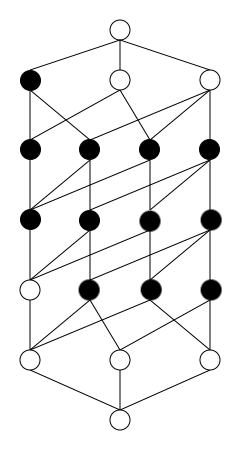
\includegraphics{counterexamplegraph.pdf}

%%%%%%%%%%%%%%%%%%%%%%%%%%%%%%%%%%%%%%%%%%%%%%%%%%%%%%%
\subsection*{Acknowledgements}
We thank Jonathan Novak (MIT) for guiding our research and providing helpful discussions.

%%%%%%%%%%%%%%%%%%%%%%%%%%%%%%%%%%%%%%%%%%%%%%%%%%%%%%%
% \bibliographystyle{plain} 
% \bibliography{myBibFile} 
% If you use BibTeX to create a bibliography
% then copy and past the contents of your .bbl file into your .tex file

\begin{thebibliography}{10}

\end{thebibliography}

\end{document}
